%%%%%%%%%%%%%%%%%%%%%%%%%%%%%%%%%%%%%%%%%%%%%%
%                insertmeeting
% 1) Title (something creative & funny?)
% 2) Date (MM/DD/YYYY)
% 3) Location (ex. Hagerty High School)
% 4) People/Committees Present 
% 5) Picture 
% 6) Start Time & Stop Time (ex. 12:30AM to 4:30PM)
%%%%%%%%%%%%%%%%%%%%%%%%%%%%%%%%%%%%%%%%%%%%%%
\insertmeeting 
	{Approaching A Peak} 
	{02/15/22} 
	{Hagerty High School}
	{James, Jensen, Samantha, Anouska, Annika, Clayton, Falon, Nathan, Ritam}
	{Images/RobotPics/robot.jpg}
	{2:30 - 4:30}
	
\hhscommittee{Software}
\noindent\hfil\rule{\textwidth}{.4pt}\hfil
\subsubsection*{Goals}
\begin{itemize}
    \item Continue refining autonomous programs. 

\end{itemize} 

\noindent\hfil\rule{\textwidth}{.4pt}\hfil

\subsubsection*{Accomplishments}
Today we were focused on fixing small problems with some of our autnomous programs. The first problem that we tackled today was inconsistency in a drive path. For the autonomous far near the carousel, we told the robot to splineTo a specific point in between the barrier and the wall to enter the warehouse. Our measurements seemed to be a bit off, so we remeasured the point with a tape measure.
The second thing we fixed today was a small bug where the arm was moving when it supposed to. Although we checked our autonomous program throughly, there were no instances where we set the arm power. After logging some debugging information and running states individually, we found that one of our movement methods was accidently calling an arm movement. 

\hhscommittee{Hardware}
\noindent\hfil\rule{\textwidth}{.4pt}\hfil
\subsubsection*{Goals}
\begin{itemize}
    \item Align and drill holes on carbon fiber sides
	\item Screw sides and wood plates together


\end{itemize} 

\noindent\hfil\rule{\textwidth}{.4pt}\hfil

\subsubsection*{Accomplishments}
Happy to finally have our long-awaited carbon fiber parts, we immediately got to work planning on how we would put it together. Because the biggest issue we would face would be lining up the sides properly to drill holes, we started out by making some templates for holes in CAD. the first thing we made was a wooden piece that had all of the important features of the top of our drivetrain. We would build the side assembly using this as the template so that software could continue working and wouldn’t be waiting for the hardware to finish. We also designed a new backplate that would also screw into the sides. We laser cut both of these parts then glued them together, simulating the dimensions of the robot (Figure \ref{fig:021522_1}). From there we used the holes on each of these plates as well as a laser cut L-shaped edge to properly position the carbon fiber sides then to drill the holes in the correct locations. After drilling all of the holes, we screed the parts together (Figure \ref{fig:021522_2}). We then repeated the process for the front, creating another plate in CAD, laser cutting it, measuring to find its correct position, and using it to drill holes on the front of the side plates then using the part to connect the carbon fiber sides (Figure \ref{fig:021522_3}). 
Now the only holes left to drill are the holes for the motor mount and bearing block. Because there is no good edge to line up a jig with, we came to the conclusion that it would be necessary to 3d print a template for the holes that could square with multiple perpendicular edges. This will give us much more precise placement of the holes. Moving into CAD, we started designing the jigs, projecting the correct hole locations onto our sketch, allowing the parts to be in the exact right spot. We used the top and side edges to align the jig, creating extrusions that will match the edges of the carbon fiber in the real world (Figure \ref{fig:021522_4}). Happy with our design, we set it up to print!

\begin{figure}[ht]
\centering
\begin{minipage}[b]{.48\textwidth}
  \centering
  \includegraphics[width=0.95\textwidth]{Meetings/February/02-15-22/2-15-22_Hardware_Figure1 - Nathan Forrer.JPG}
  \caption{The combined pieces}
  \label{fig:021522_1}
\end{minipage}%
\hfill%
\begin{minipage}[b]{.48\textwidth}
  \centering
  \includegraphics[width=0.95\textwidth]{Meetings/February/02-15-22/2-15-22_Hardware_Figure2 - Nathan Forrer.JPG}
  \caption{Screwing the parts together}
  \label{fig:021522_2}
\end{minipage}
\end{figure}

\begin{figure}[ht]
\centering
\begin{minipage}[b]{.48\textwidth}
  \centering
  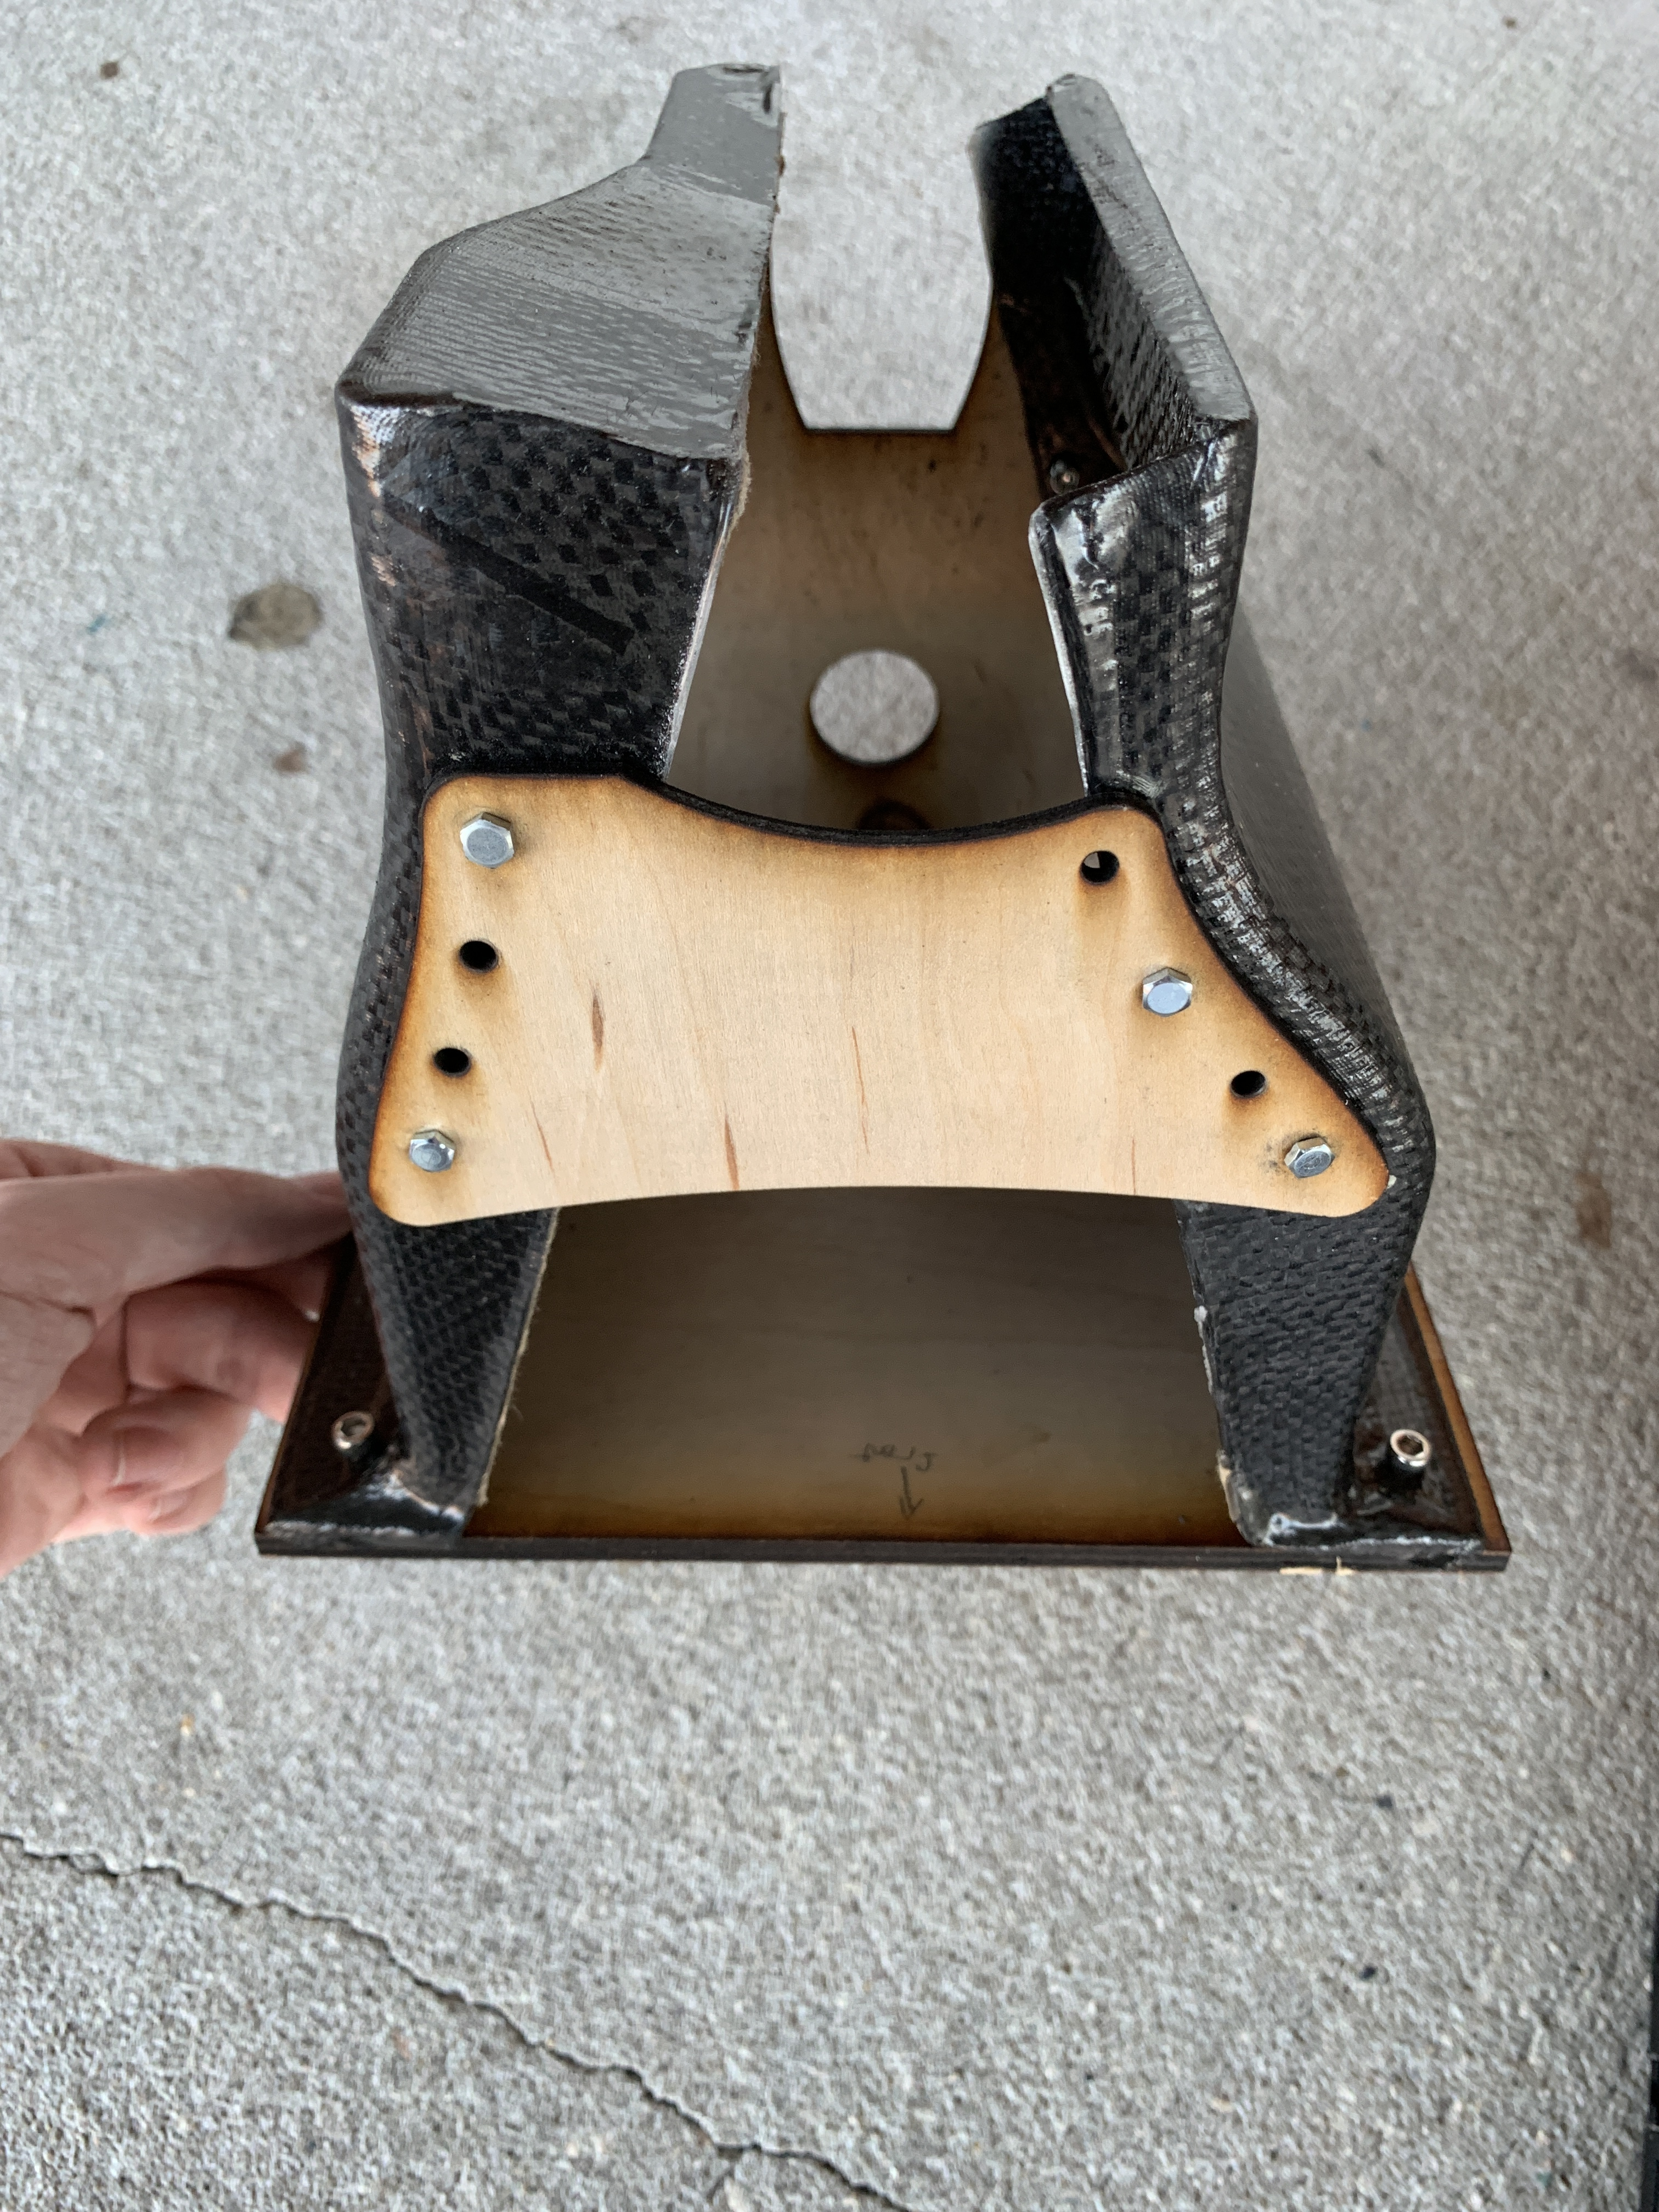
\includegraphics[width=0.95\textwidth]{Meetings/February/02-15-22/2-15-22_Hardware_Figure3 - Nathan Forrer.JPG}
  \caption{Connecting the part to the carbon fiber}
  \label{fig:021522_3}
\end{minipage}%
\hfill%
\begin{minipage}[b]{.48\textwidth}
  \centering
  \includegraphics[width=0.95\textwidth]{Meetings/February/02-15-22/2-15-22_Hardware_Figure4 - Nathan Forrer.JPG}
  \caption{Extrusions to match the edges of the carbon}
  \label{fig:021522_4}
\end{minipage}
\end{figure}




\whatsnext{
\begin{itemize}
    \item Drill holes for motor and bearing block
	\item Screw in motor and bearing block

\end{itemize} 
}

